\section{Design Summary}

The design of this device encompasses three main sections; the DAW, the Autofill Feature,
and the Keyboard interface. The integration of these three sections will create the final
product. The DAW will manage the MIDI files and display any changes that occur from the
keyboard or Autofill feature. The Autofill feature will take the current MIDI file from
the daw and generate suggestions for imporovements and future notes to be added to the
MIDI file. The Keyboard will be the method of imputting new notes or chords to the DAW and
subsequently the MIDI files. The combination of all three of these task is what our design
seeks to accomplish.

\subsection{Keyboard}

The keyboard will act as the physical interface that users interact with when inputting to
the DAW. This section encompasses the metronome, keys, volume control, record, and play
features. Each input affects the resulting Audio Playback and subsequently gives that data
to the DAW, which will act as the main controller of the entire system. Figure 4
encompasses this idea in a compressed and streamlined graphic.

\begin{figure}[h!]
  \centering
  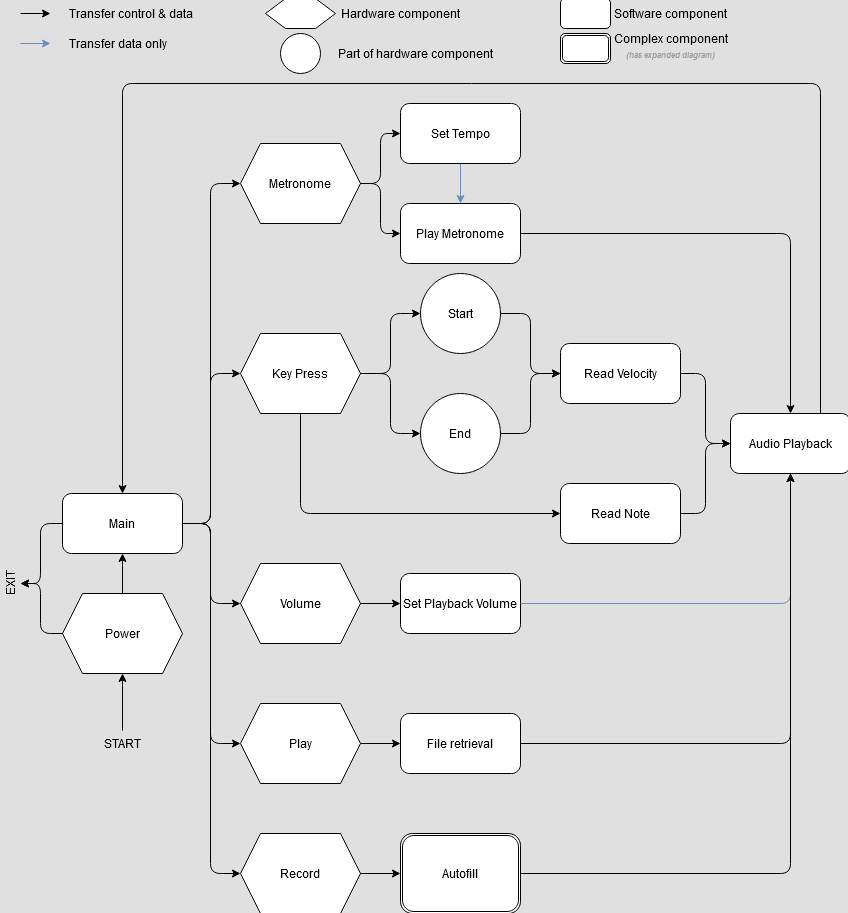
\includegraphics[width=\linewidth]{image/Keyboard.png}
  \caption{The overall structure of the project}
  \label{fig:keyboard_diagram}
\end{figure}

\subsection{DAW}
The DAW will act as the central location where MIDI files will be created and stored. It
will take inputs from the Keyboard and give complete MIDI files to the Autofill AI. It
will also allow the user to adjust and place notes that they believe require adjustment.
The DAW feature will allow for a centralized and streamlined processing of inputs and
outputs as well as a interface for the user to interact with the MIDI controller.

\begin{figure}[h!]
  \centering
  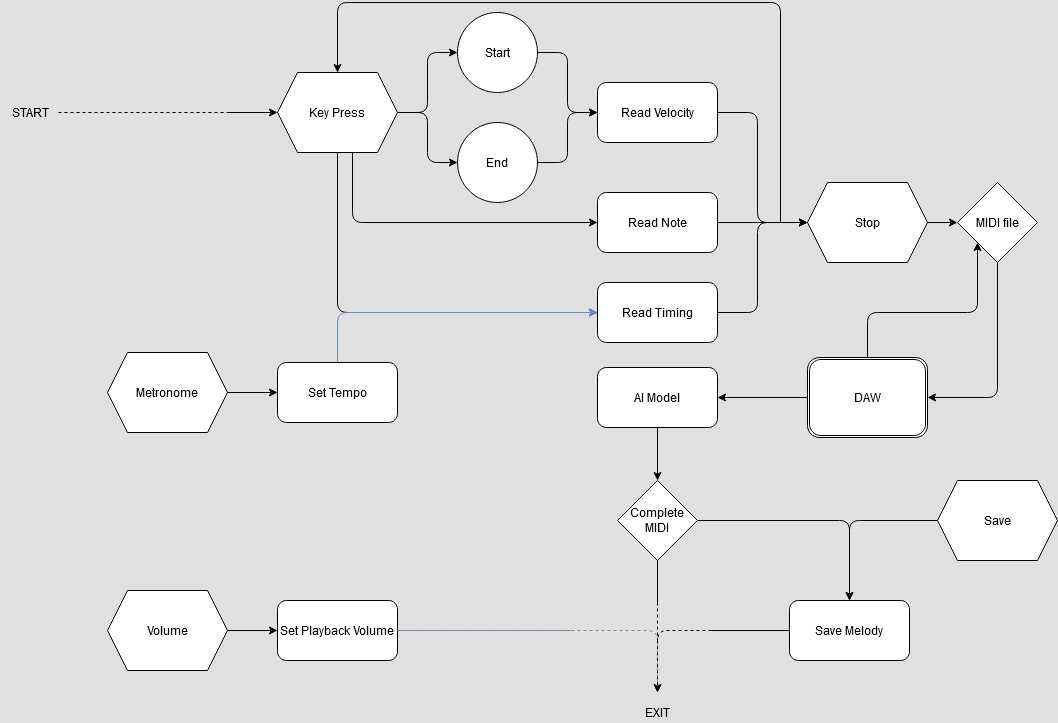
\includegraphics[width=\linewidth]{image/Autofill.png}
  \caption{Structure of the melody autofill component}
  \label{fig:autofill_diagram}
\end{figure}

\subsection{Autofill Feature}

The autofill feature is the main focus of this project as it is the central idea of our
initial design meeting. The Autofill feature will extract the MIDI file generated by the
DAW and create a number of subsequent files to help the user compose melodies of
symphonies representative of the selected genre. This will be accomplished using a trained
AI that is capable of further improvements via thirdparty connections and processing. 

\begin{figure}[h!]
  \centering
  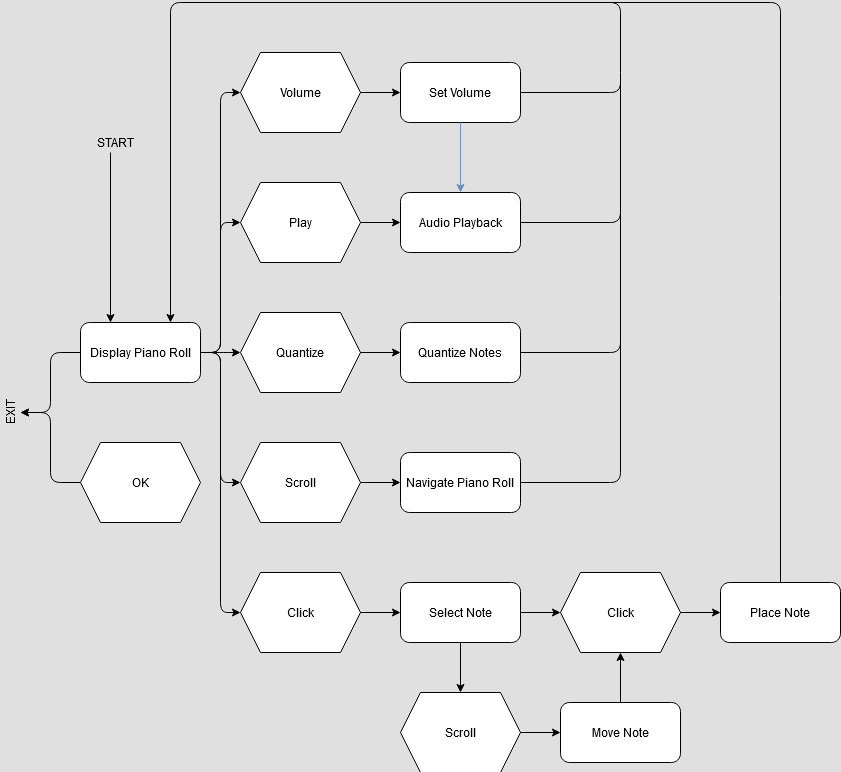
\includegraphics[width=\linewidth]{image/DAW.png}
  \caption{Structure of the MIDI editing component}
  \label{fig:daw_diagram}
\end{figure}
\clearpage
